%!TEX root = _thesis.tex
\chapter{手指使用量常時計測の理論と計測ステム構築}

\section{手指使用量の常時計測方法}
既存の手法の問題点を考察すると,手指使用量の常時計測に向いた計測手法は以下の要件を満たす必要がある.

\begin{itemize}
 \item 計測機器が持ち運びやすい
 \item ノイズに対してロバストである
 \item 定量的である
 \item ユーザへの負担が少ない
\end{itemize}

そのため,これらの要件を満たし,手指使用量が計測可能なウェアラブルデバイスの開発を目的とする.計測機器が持ち運びやすいを満たすには,軽量でコンパクトな計測機器が求められる.



\section{指の関節角度計測}
本研究の手指使用量の測定手法は,指の関節角度の変化が,指の使用量を反映するという仮定に基づく.関節角度の変化の推定には,ウェアラブルデバイスに搭載された赤外線距離センサを用いる.本デバイスは指の基節に装着して使用し,赤外線距離センサで,デバイスから中節までの距離を常時計測する.式(1)の関数を用い,測定された距離を指の関節角度に変換し,指の使用量を測る.距離を角度変換する模式図をFig.\ref{fig:principle}に示す.

\begin{figure}[H]
  \centering
  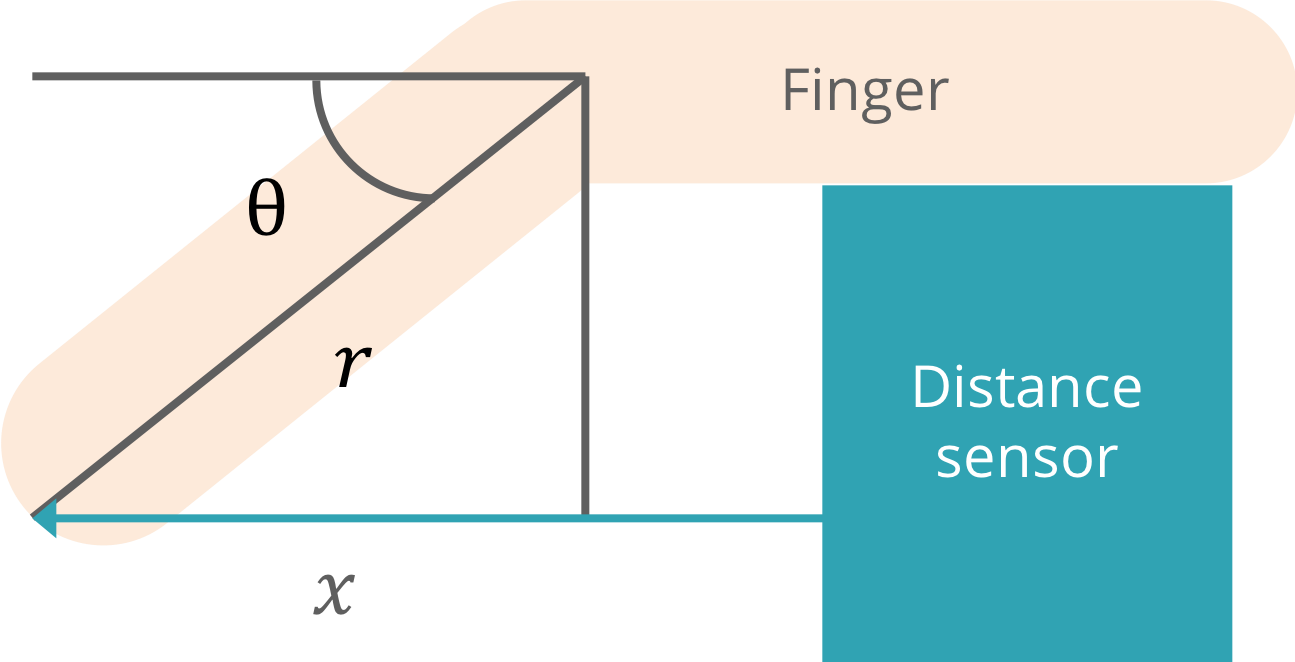
\includegraphics[width=0.8\linewidth]{fig/principle}
  \caption{Measurement principle}
  \label{fig:principle}
\end{figure}

\begin{equation}
\theta = \cos^{-1} \frac{x}{r}
\label{eq:theta}
\end{equation}


ここで,$r$は第二関節から指先までの長さ,$x$は最大屈曲時からの変化距離,$\theta$は最大伸展時からの変化角度である.
$r$はデバイス使用前に物差しやスケール等を用い測定しておく必要がある.$x$は本デバイスの赤外線距離センサによって測定,推定する.この$r,x$の二つのパラメータと式\ref{eq:theta}を用いることで,関節角度$\theta$を導出する.



\section{ウェアラブルデバイスのハードウェア}
本デバイスは加速度計と赤外線距離センサの2つのセンシング部と,センシングされたデータを格納するデータ記録部からなるウェアラブルデバイスである.
本研究で開発したウェアラブルデバイスをFig.\ref{fig:device}に示す.
\begin{figure}[H]
  \centering
  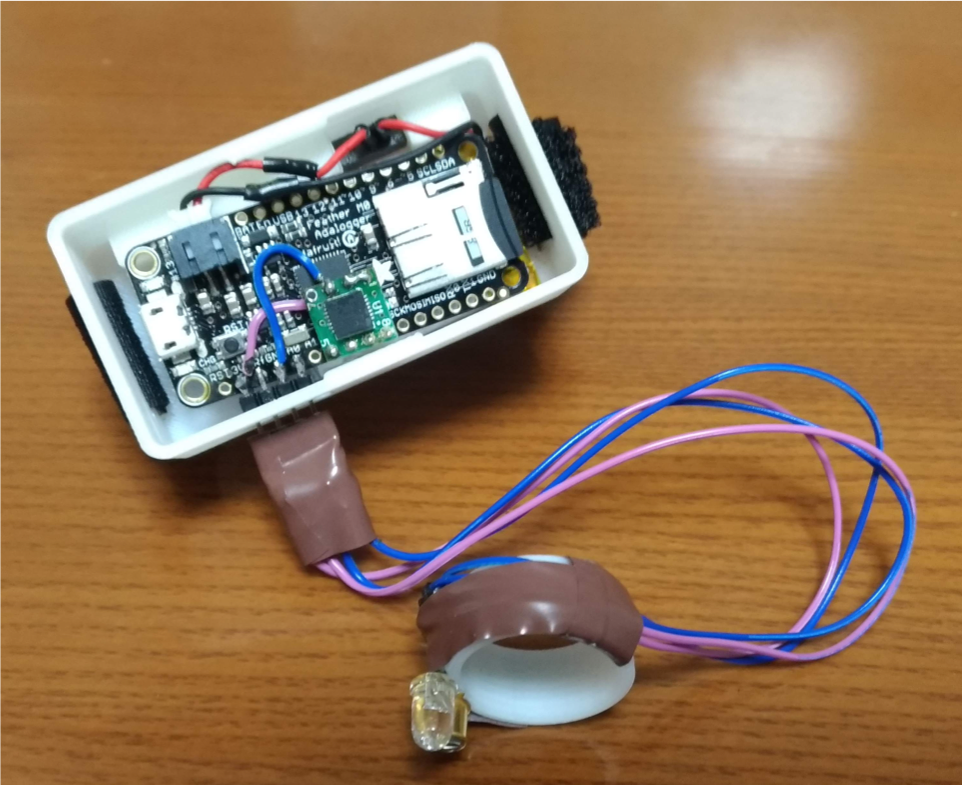
\includegraphics[width=0.8\linewidth]{fig/fal6}
  \caption{Hardware of the wearable device}
  \label{fig:device}
\end{figure}


本デバイスの指輪型の装着部分及び,バッテリーとマイコン基盤を収納するためのケースを3DCAD(Fusion 360)で設計し,3Dプリンタ(Dimension 1200es)で印刷し作成した.


\subsection*{センシング部}
距離計測と加速度計測を行うため,赤外線距離センサと加速度計の二つのセンサを利用した.
\subsubsection*{赤外線距離センサ}
指関節角度の変化をセンシングするため赤外線距離センサを使用した.
赤外線距離センサは発光ダイオード(Osram SFH4550)とフォトトランジスタセンサ(Honeywell SD5410)で構成されている.
赤外線距離センサは発光ダイオードが発光した際に出た光をフォトトランジスタで受光することで,距離を計測するセンサである.
フォトトランジスタの受光量は,ランベルトの反射の性質を有し,光が反射物に反射し受光素子に当たるまでの距離と角度,反射物の反射率により決定される(逆自乗の法則).そのため,センシングキャリブレーションを行った.センシングキャリブレーションに関しては後述する.
外部から入る光によるノイズを抑えるため,発光ダイオードとフォトトランジスタはそれぞれ6$^\circ$と12$^\circ$の狭い視覚野を持つパーツを選定した.手指の関節角度を測定するため,赤外線距離センサを指に取り付ける必要がある.
しかし,直接,テープや手袋などで赤外線距離センサを,ユーザの指に取り付けると,デバイスの装着や取り外しが煩雑になり,
ユーザへの負担が大きくなる問題が生じる.そのため,指輪型のハードウェアへ赤外線距離センサを取り付けた.これにより,ユーザにかかるデバイスの着脱による負荷を低減した.指輪型のハードウェアは3次元コンピュータ支援設計ソフトウェア(Three-dimensional computer-assisted drafting:3DCAD)で設計後,3Dプリンタを用いて作成した.

指輪型ハードウェアの大きさが,ユーザの指の太さと合っていない場合,センサのずれやユーザビリティの低下等の問題が発生する.
ユーザごとに指の太さが異なることが予想されるため,指輪の直径が異なる複数の指輪型のハードウェアを作成した.
AIST\cite{}を参考に,日本人の平均的な食指の直径である,18,19,20,21mmの直径を持つ指輪型ハードウェアを作成した.

\begin{figure}[H]
  \centering
  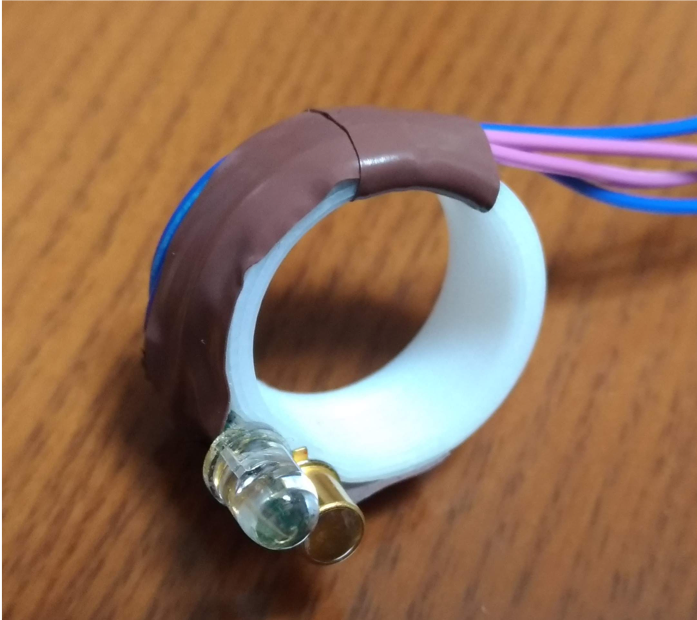
\includegraphics[width=0.8\linewidth]{fig/fal7}
  \caption{Infrared distance sensor consists of LED and Phototransistor}
  \label{fig:distance sensor}
\end{figure}

赤外線距離センサはマイクロコンピュータとワイヤーで接続されており,マイクロコンピュータから給電を行なっている.また,フォトトランジスタがセンシングしたデータをマイクロコンピュータへ出力している.以下のFig.\ref{fig:circuit}に,赤外線距離センサとマイクロコンピュータ(Arduino)の接続を示す.

\begin{figure}[H]
  \centering
  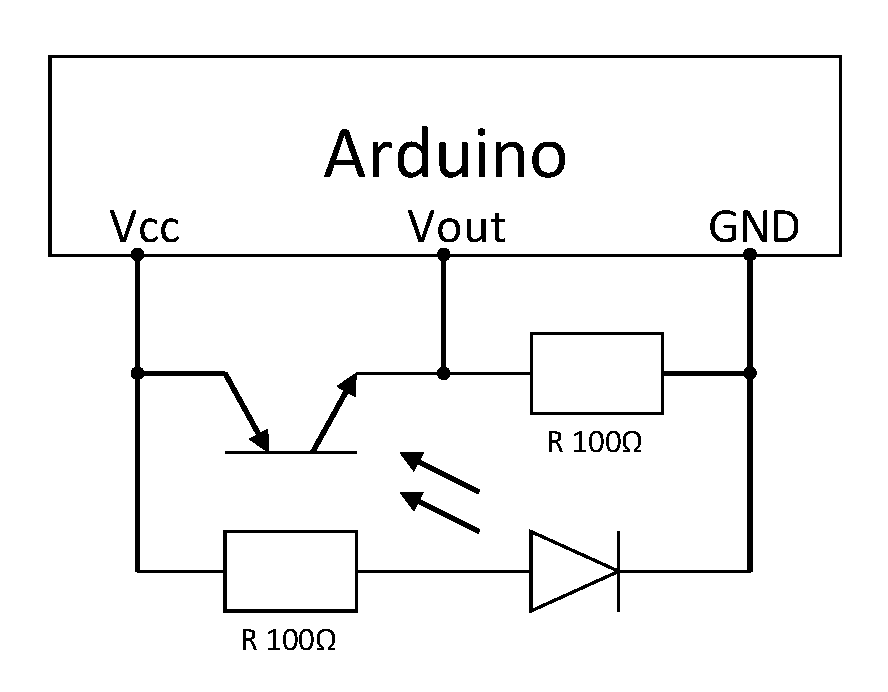
\includegraphics[width=0.5\linewidth]{fig/test}
  \caption{Circuit of the wearable device}
  \label{fig:circuit}
\end{figure}



\subsubsection*{三軸加速度センサ}
さらに,マイコン基盤に三軸加速度センサ(KXR94-2050)を追加した.

\begin{figure}[H]
  \centering
  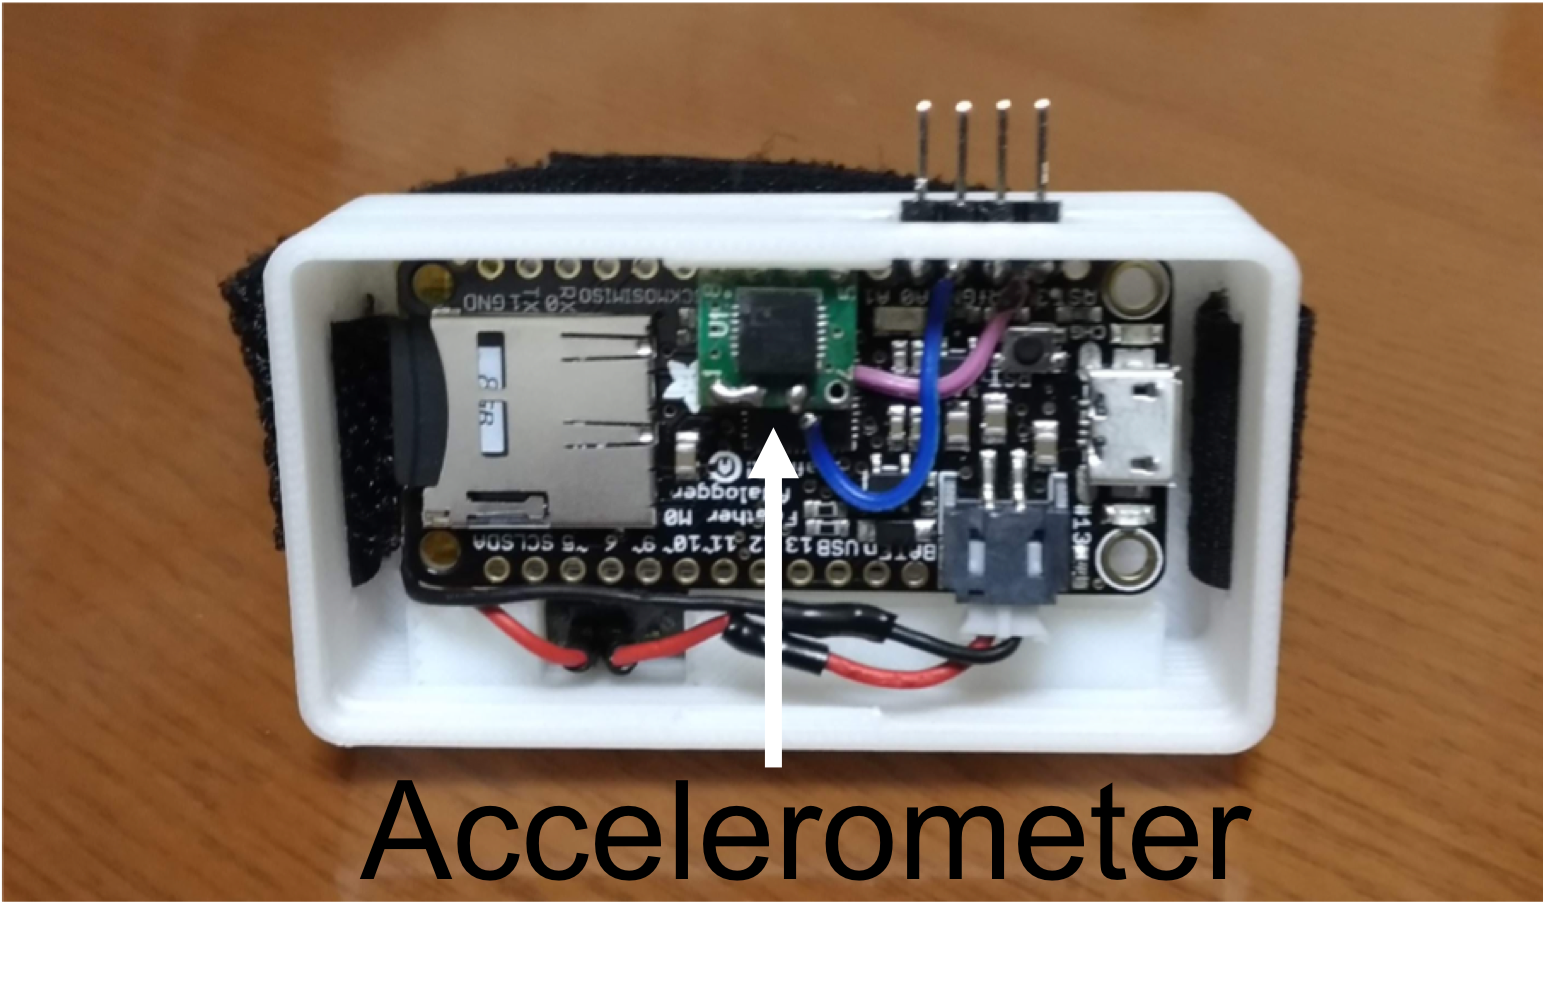
\includegraphics[width=0.5\linewidth]{fig/accelerometer}
  \caption{Accelerometer}
  \label{fig:accelerometer}
\end{figure}

\subsection*{データ記録部}
\subsubsection*{SD card}
データ記録のため,マイコン基盤(Adafruit Faether M0)と32GBのSDcardを使用する.
赤外線距離センサと加速度センサからの信号は,信号の入力時間とともにマイコン基盤に接続されたMicro sdカードへ保存される.コンピュータへUSB2.0 A Male Microケーブルで接続することで,本デバイスのリポバッテリーの充電と,Micro sdカードに記録されたデータの転送が可能である.


\begin{figure}[H]
  \centering
  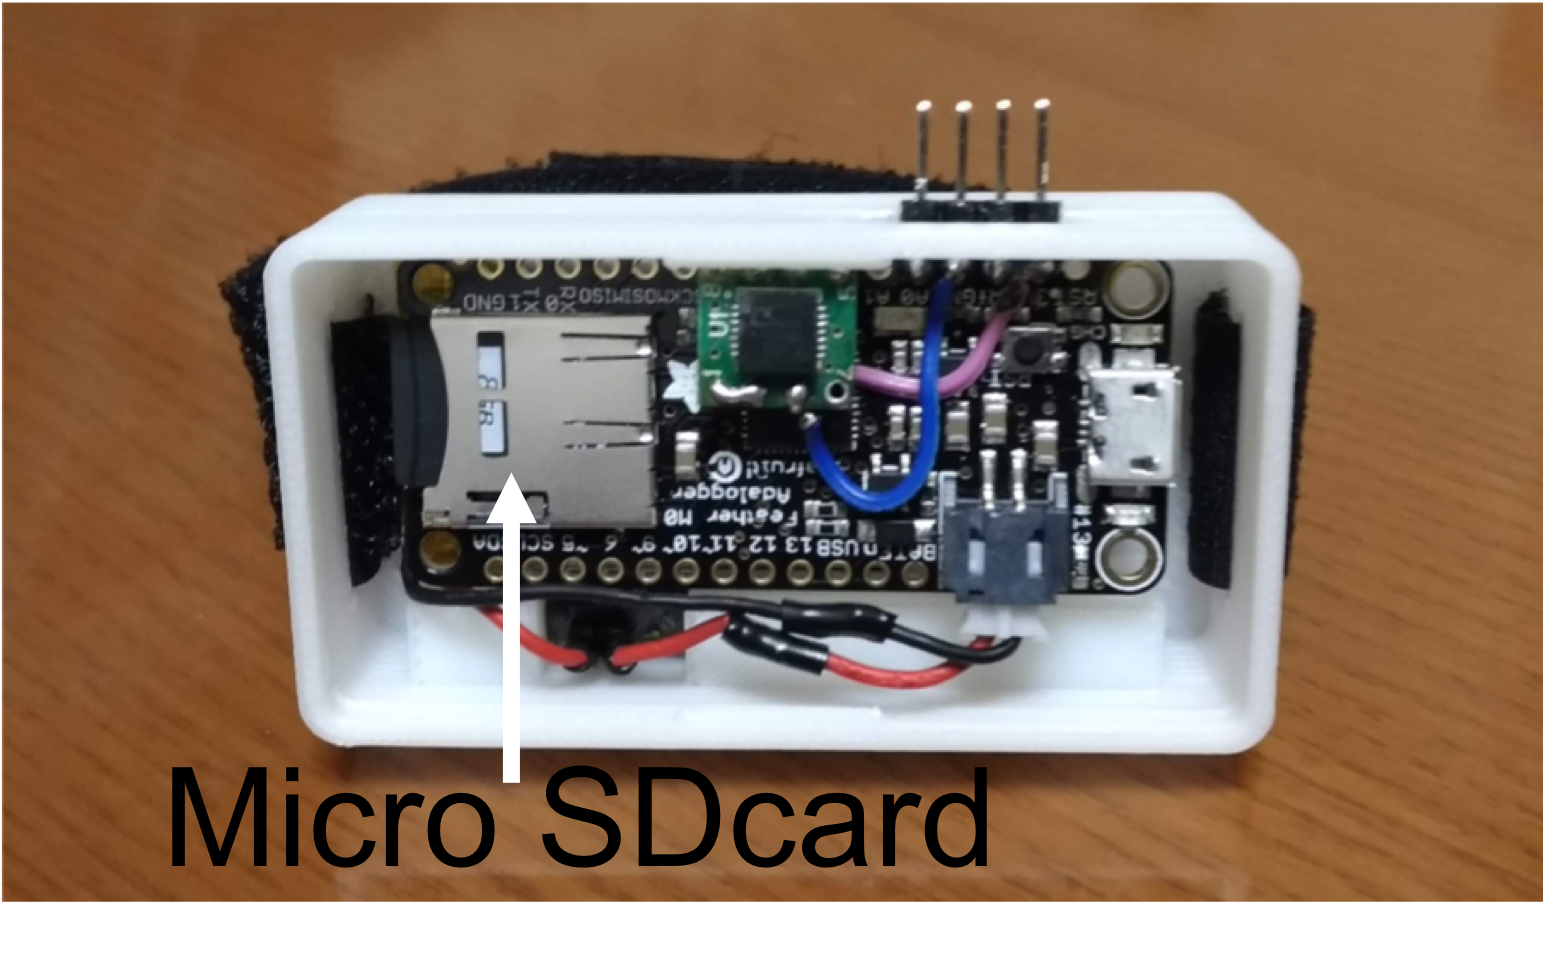
\includegraphics[width=0.5\linewidth]{fig/sdcard}
  \caption{Micro SDcard}
  \label{fig:sd card}
\end{figure}


\subsubsection*{LiPO battery}
デバイスの電源として3.7V,400mAhのリポバッテリーを利用し,これにより24時間以上の連続電源供給が可能である.
\begin{figure}[H]
  \centering
  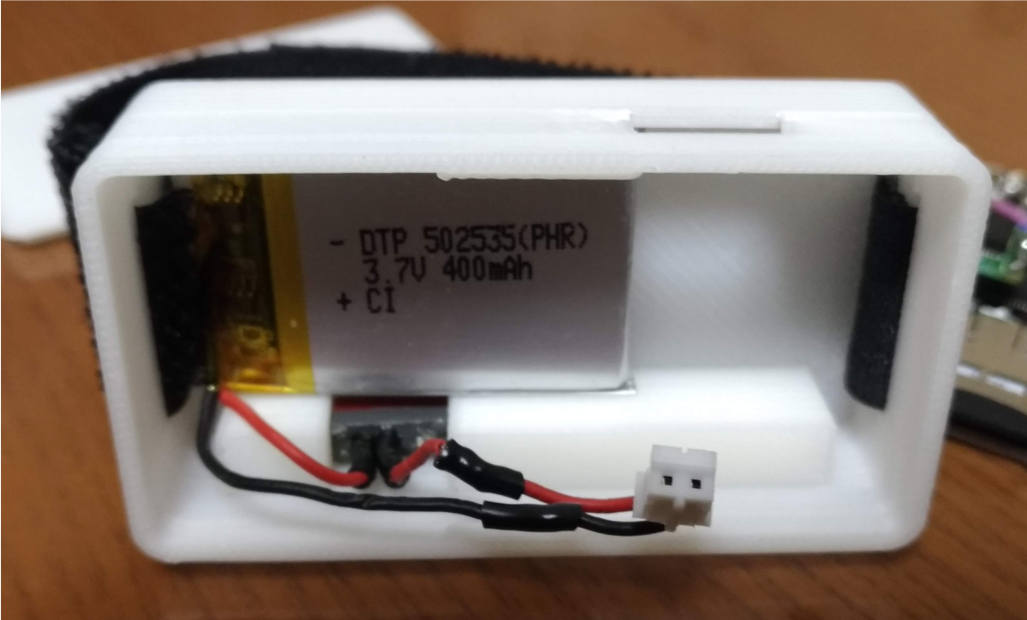
\includegraphics[width=0.5\linewidth]{fig/battery}
  \caption{A LiPO battery}
  \label{fig:battery}
\end{figure}



\subsection*{ウェアラブルデバイスの使用法}
本デバイスに取り付けられたスイッチをオンにすると,赤外線距離センサと加速度センサの記録を開始する.スイッチをオフにするまで連続計測,記録する.データはCSVファイルでSD card内に保存される.本デバイスに記録されたデータは,コンピュータと本デバイスのdeta-logging boardのArduinoをUSBケーブルで直接繋ぐか,Micro SDcardをコンピュータに移すことで,アクセスが可能である.

本デバイスの装着方法をFig\ref{fig:ring}に示す.指輪型のセンシング部は,食指の第二関節に装着し,ストレージ部は手首にマジックテープを使用し取り付ける.



\begin{figure}[H]
  \centering
  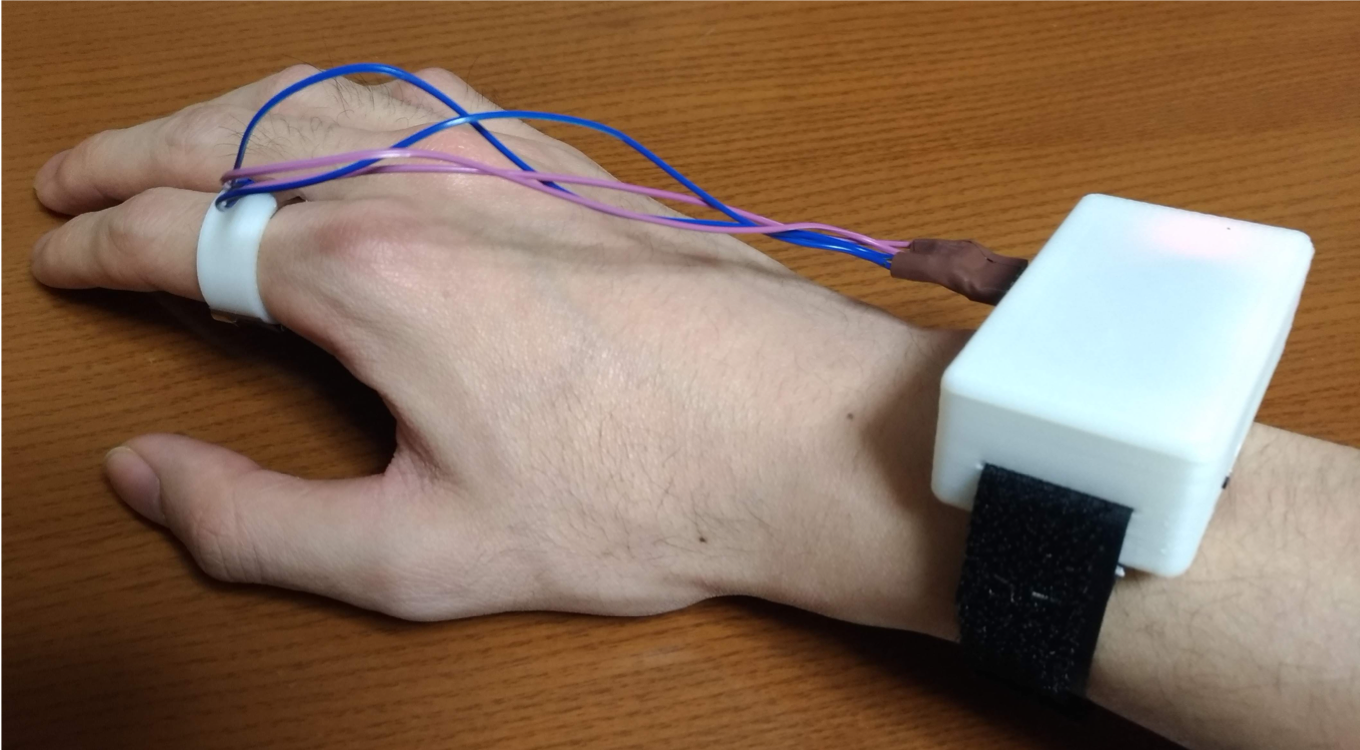
\includegraphics[width=0.8\linewidth]{fig/fal4.png}
  \caption{Ring worn on the index finger and Strage worn on the wrist}
  \label{fig:ring}
\end{figure}


\section{センシングキャリブレーション}
赤外線距離センサは物体に反射し,フォトトランジスタで受光した赤外線の強度を計測することで,距離を推定する.
しかし,同じ距離であっても赤外線が反射する物体によっては,違う
受光量となる場合がありえる.これは物体によって光の反射率が違い,同じ距離で計測したとしても,フォトトランジスタで受け取る受光量が違ってくるためである.つまり,人によって,指の長さや皮膚の色が違うため,同じセンサ値であっても,本来の距離が変わる問題がある.この問題を解決するために,被験者ごとに皮膚の反射率を調べることが望ましいが,本システムは日常生活での使用を目的としており,キャリブレーションがユーザに負荷をかけないことが求められる.
そのため,本システムでは計測される距離と受光量の関係を求め,キャリブレーションが可能な方法を提案する.キャリブレーションには以下の3つのパラメータを用いる.

\begin{itemize}
 \item デバイスを装着する指の長さ
 \item 指伸展時のセンサ情報
 \item 指屈曲時のセンサ情報
\end{itemize}

得られたセンサ情報と指の長さのデータにより,線形近似を行い,ユーザごとのキャリブレーションを行った.




\section{センシング情報の処理方法}
デバイスにより取得できる電圧値は,ノイズを含んでいるため,ノイズの除去を行った.
また,ノイズの除去はバターワイスローパスフィルターにより,10hz以上の周波数を持つシグナルをカットオフすることで行った.赤外線距離センサのセンシングデータから指間接角度を推定する際、いくつかの信号処理を行った.さらに、指の使用量へ変換する処理も行った.それら処理を以下に示す.

\begin{enumerate}
 \item 100Hzのサンプリングレートをもつセンシングデータを10Hzにダウンサンプリングした
 \item  ローパスフィルタにより、ノイズデータを除去した.1次元線形回帰により、センシングデータを,センサから指までの距離へ変換した.
 \item 関節角度が90度,0度のときのセンシングデータを利用し,キャリブレーションを行った
 \item 式\ref{eq:theta}により,距離を角度に変換した
 \item 角度を時間微分し,角度時間の変化角度を導出した
 \item 変化角度の絶対値をとり,タスクごとの指の使用量(タスクの合計変化角度)を導出した.
\end{enumerate}
